\documentclass[a4paper]{article}
\usepackage[spanish]{babel}
\title{Taller 1}

\usepackage[utf8]{inputenc}
\usepackage{caratula}
\usepackage{graphicx}
\usepackage{color}
\usepackage{listings}
\usepackage{float}


\setlength{\leftmargin}{2cm}
\setlength{\rightmargin}{2cm}
\setlength{\oddsidemargin}{-1cm}
\setlength{\evensidemargin}{-1cm}
\setlength{\topmargin}{-1cm}
\setlength{\textwidth}{18cm}
\setlength{\textheight}{25cm}

\usepackage{fancyhdr}
\pagestyle{fancy}
\fancyhf{}
\fancyhead[LO,LE]{\scriptsize Trabajo Práctico N$^{\circ}$2}
\fancyhead[RO,RE]{\scriptsize Mancuso, Mataloni, Gonzalez}
\fancyfoot[CE,CO]{\thepage}
\renewcommand{\footrulewidth}{0.4pt}

\usepackage[pdftex, bookmarks=true, colorlinks, citecolor=black, linkcolor=black]{hyperref}
\usepackage{multirow}

\begin{document}

\materia{Teoría de las Comunicaciones}
\submateria{Segundo Cuatrimestre de 2012}
\titulo{Taller de Capa de Transporte}
\grupo{Taller N$^{\circ}$3}

\integrante{Mancuso, Emiliano}{597/07}{emiliano.mancuso@gmail.com}
\integrante{Mataloni, Alejandro}{706/07}{amataloni@gmail.com}
\integrante{Gonzalez, Matias}{453/07}{curtu\_infinito73@hotmail.com}

\maketitle

\newpage

\addcontentsline{toc}{section}{Índice}

% Main project


\newpage


\section{Primera consigna}


\section{Segunda Consigna}

\subsection{Banner Grabbing y servicios suceptibles:}
Como se explico en clase  Banner Grabbing es una tecnica en la cual se obtiene informacion a traves de las aplicaciones que corren en los distintos puertos de un host. La informacion obtenida puede ser
versiones y nombre de las aplicaciones, esta inforamcion puede ser utilizada para detectar o inferir el sistema operativo o para explotar las vulnerabilidades de la aplicacion en si.

Debido a que la tecnica trabaja sobre aplicaciones, son varios los servicios que deberian ser vulnerables. Una de las primera ideas que tuvimos es que todos los puertos dedicados a aplicaciones
podrian ser suceptibles. La realidad nos mostro que eso no es cierto, en la mayoria de los casos los host no implmentan todos, ni muchos, de los servicios disponibles. 

Por esta razon es que investigamos un poco y descubrimos que  los servicios suceptibles esta tecnica, mas comunes suelen ser:
\begin{itemize}
\item Web/Aplicaciones Web puerto 80
\item FTP (transferencia de archivos) puerto 21
\item SMTP (mail) puerto 25
\end{itemize}


Pero nuestro primer pensamiento no era del todo errado como Banner Grabbinng se utiliza para obtener informacion sobre servicios tambien existen otros que son suceptibles, pero la suceptibilidad depende
varios factores como: uso del host, seguridad del mismo, etc. Los servicios, y la "suceptibildiad"\ de los mismos, no suelen ser tan comunes. Algunos de ellos son:

\begin{itemize}

\item DNS puerto 53
\item MYSQL (base de datos) 3306
\item POSTGRE (base de datos) 5432
\item POP3 (mail) 110

\end{itemize}


Banner Grabbing se puede realizar de muchas maneras como utilizar alguna de las herramientas de testeo y analisis vista en clase, utilizando alguna aplicacion de conexion como telnet. Debido que al 
establecer la conexion las aplicaciones presentan inforacion sobre las ellas, entonces lo unico que se necesita es cambiar el puerto al que nos conectamos en el host para que los distintos servicios nos
brinden informacion.

Aunque dependiendo de el servicion del que se esta queriendo obtener informacion, tambien se pueden utilizar aplicaciones para el trabajo con esos protocolos, como puede ser:
\begin{itemize}
\item ftp por linea de comando en linux.
\item Navegadores.
\item clientes de mail desde consola.
 \end{itemize}
 
 En algunos casos esta opcion tambien puede ser mas divertida.
 
 En otros casos como el DNS, que en realdiad no tiene un "banner" para agarrar, se debe usar la herramiento dig para obtener la version.
 
\subsection{Implementaciones de Captura}
 
Como se menciona antes la tecnica de Banner Grabbing se puede realizar de varias maneras con distintas herramientas, conectandose a un host y probando en los distintos puertos.

\begin{itemize}
\item Telnet: \textit{telnet $<$host$>$  $<$port$>$}

\item Netcat: \textit{nc $<$host$>$ $<$port$>$}
\end{itemize} 

\clearpage

Tambien se puede realizar con herramientas propias de cada aplicacion de la que querramos obtener la informacion.

\begin{itemize}
\item FTP: \begin{itemize}
			\item \textit{ftp $<$host$>$}
			\item Comenzar la aplicacion ingresando en consola \textit{ftp}, dentro de la consola ftp escribir \textit{open $<$host$>$}
			\end{itemize}
			
\item SSH: \textit{ssh $<$host$>$}, esta opcion no siempre es la mejor porque suele dejar huellas de los ingresos.

\item DNS: \begin{itemize}
			\item \textit{dig -c CH -t txt version.bind @$<$host$>$}, obtener la version simple
			\item \textit{dig -t tct -c chaos version.bind @$<$host$>$}, cuando se quiere acceder a la version a traves de clase CHAOSNET.
			\end{itemize}
			
\end{itemize}


\section{Tercera consigna}

Corrimos el comando nmap contra 3 hosts locales con diferentes sistemas operativos. La herramienta logro identificar satisfactoriamente a 2 de ellos (Apple Mac OS X 10.7.0 y Windows XP) pero no pudo reconocer a Windows 7. Suponemos que esto se debe a que al ser un sistema relativamente nuevo, todavia no se cuenta con mucha informacion para reconocerlo facilmente. \\


Capturamos el trafico con \textit{Wireshark} y pudimos verificar las distintas pruebas que ejecuta nmap.\\

Para el proceso de escaneo de puertos utiliza la tecnica de syn scan. Con esto se obtienen los diferentes puertos en estado \textit{open} o \textit{close}, los cuales luego utiliza para realizar varios tests.


\begin{figure}[H]
  \centering
  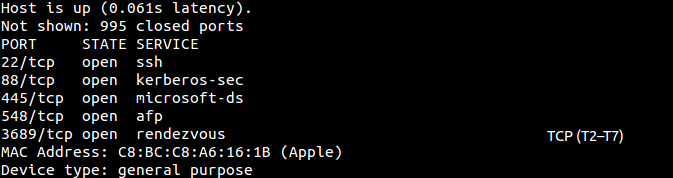
\includegraphics[scale=0.60]{graficos/macPorts.png}
  \caption{Resultado syn scan Mac OS X}
\end{figure}  

\begin{figure}[H]
  \centering
  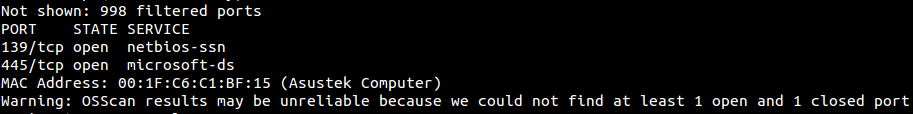
\includegraphics[scale=0.60]{graficos/windowsPorts.png}
  \caption{Resultado syn scan Mac OS X}
\end{figure}  

Las pruebas que pudimos observar:

\begin{itemize}

\item ICMP echo (ie): Se envian 2 paquetes ICMP con algunos parametros fijos. En el primero se setea el DF flag de la capa IP,el TOS (tipo de servicio) en 0, el codigo de ICMP es 9, el numero de secuencia es 295.\\
En el segundo se setea el TOS en 4, el codigo en 0, y el ICMP requestId y numero de secuencia se incrementan en 1 de los valores del primer paquete.

\item TCP explicit congestion notification (ECN): Se envia un paquete TCP con los siguientes flags a uno de los puertos en estado open: SYN, ECN, CWR.

\item UDP (U1): Se envia un paquete UDP a un puerto en estado close. Se setea el IP ID en 0x1042 y se repite el caracter  \textit{C} en el campo de datos. 

\end{itemize}






\end{document}
